\documentclass[a4paper, 11pt, notitlepage]{article}
\addtolength{\hoffset}{-1cm}
\addtolength{\textwidth}{2cm}
\usepackage[utf8]{inputenc}
\usepackage[frenchb]{babel}
\usepackage[T1]{fontenc}

\usepackage{multicol}
\usepackage{listings}
\usepackage{graphicx}
\usepackage{hyperref}

\usepackage{color}
\definecolor{lightgray}{rgb}{.9,.9,.9}
\definecolor{darkgray}{rgb}{.5,.2,.2}
\definecolor{purple}{rgb}{0.65, 0.12, 0.82}
\definecolor{brown}{RGB}{140, 0, 0}

\lstnewenvironment{OCaml}
                  {\lstset{
                      language=[Objective]Caml,
                      breaklines=true,
                      showstringspaces=false,
                      commentstyle=\color{red},
                      stringstyle=\color{darkgray},
                      identifierstyle=\ttfamily,
                      keywordstyle=\color{blue},
                      basicstyle=\footnotesize,
                      escapeinside={/*}{*/},
                      %xleftmargin=0.08\textwidth
                    }
                  }
                  {}
\lstnewenvironment{OCamlEx}
                  {\lstset{
                      language=[Objective]Caml,
                      breaklines=true,
                      showstringspaces=false,
                      commentstyle=\color{red},
                      stringstyle=\color{darkgray},
                      identifierstyle=\ttfamily,
                      keywordstyle=\color{blue},
                      basicstyle=\footnotesize,
                     escapeinside={/*}{*/},
                      frame=single,
                      numbers=left,
                      %xleftmargin=0.08\textwidth
                    }
                  }
                  {}
\newcommand{\class}{\ttfamily\textit{class}}
\newcommand{\interface}{\ttfamily\textit{interface}}
\newcommand{\name}{\ttfamily\textit{name}}
\newcommand{\package}{\ttfamily\textit{package}}
\newcommand{\ident}{\footnotesize\textbf{ident}}
\newcommand{\fun}[1]{\ttfamily\textbf{#1}}

\lstdefinelanguage{idlgrammar}{
  morekeywords={package,abstract,extends,class,implements,static,final,<ini>,interface,callback,array,[,],{,},
    name ,void,boolean,byte,char,short,int,long,float,double,string},
  alsoletter=[]{},
}
\lstnewenvironment{idl}
                  {\lstset{
                      language=idlgrammar,
                      breaklines=true,
                      showstringspaces=false,
                      keywordstyle=\ttfamily\color{blue},
                      identifierstyle=\ttfamily\textit,
                      basicstyle=\footnotesize,
                     escapeinside={(*}{*)},
                      %xleftmargin=0.08\textwidth
                    }
                  }
                  {} 



%%%%%%%%%%%%%%%%%%%%%%%%%%%%%%%%%%%%%%%%%%%%%%%%%%%%%%%%%%%%%%%%%%%%%%%%%%%%%%



\title{
  \huge L'interopérabilité entre OCaml et Java\\
}
\author{
  Béatrice Carre \\
  beatrice.carre@etu.upmc.fr \\
  \\
  encadrants : Emmanuel Chailloux, Xavier Clerc et Grégoire Henry \\
}

\begin{document}
\maketitle
\tableofcontents
\newpage
\section*{Introduction}
\addcontentsline{toc}{section}{Introduction}
Il arrive d'avoir envie de réutiliser des structures
écrites dans un certain langage sans avoir à les réécrire complètement.
Il peut arriver de vouloir d'utiliser l'efficacité et
l'élégance du style fonctionnel d'Ocaml pour les calculs d'un
programme mais aussi la portabilité du style objet de Java et la
diversité de son API.

C'est pourquoi l'interopérabilité est un problème intéressant.
L'interopérabilité engenre beaucoup de questions sur la gestion de
plusieurs éléments :
le cohérence des types d'un langage à l'autre,
la copie ou partage des valeurs d'un monde à l'autre,
le passage des exceptions,
la gestion automatique de la mémoire (GC), 
et celle des caractéristiques de programmation pas forcément gérées dans les
deux langages.

Deux études ont déjà été réalisées pour l’interopérabilité entre
Ocaml et Java à travers leur modèle object respectif :

\emph{O’Jacaré} conserve les runtimes des deux langages (GC,
Exceptions, ...) et les fait communiquer avec l'aide de CamlJava, TODO.

\emph{OCaml-java
  2.0} utilise un seul runtime, celui de Java, en compilant les programmes OCaml en byte-code Java. TODO.
\newline

L'idée est de profiter des deux approches, l'accès direct à toute
l'API Java grâce à OCaml-Java, et l'accès à d'autres classes définies
par le programmeur intéressé, en générant le code nécessaire à cet
accès grâce à O'Jacaré, et le tout en gardant qu'un seul runtime, la JVM.

Après l’étude des deux outils, le projet consiste à engendrer pour
ocaml-java les fichiers d’encapsulation d'O’Jacaré. Ce
portage est réalisé en OCaml étant donné qu'il reprend ce qui
a déjà été développé pour O’Jacaré.
\newline

Dans ce rapport, nous décrivons le schéma global avec ses avantages du
générateur de code d'O'Jacaré, et celui du compilateur d'Ocaml-Java,
pour détailler ensuite les modifications apportées à la génération
d'interfaces, adaptée pour une encapsulation utilisable par le
compilateur d'OCaml-Java. 
Pour finir, un exemple d'application accompagnée d'un
test de performance sera présenté.










\newpage

\section{L'interopérabilité entre OCaml et Java}

%%%%%%%%%%%%%%%%%%%%%%%%%%%%%%%%%  1.1  O'Jacaré   %%%%%%%%%%%%%%%%%%%%%%%%%%%%%%%%%%%

\subsection{O'Jacaré, un générateur de code d'interface}
O'Jacaré génère le code nécessaire à l'encapsulation des classes
définies dans un IDL, pour permettre aux interface avec C de chacunes
de comminuquer.

\subsubsection{Principe global}
O'Jacaré génère des fichier permettant à CamlJava de faire communiquer les deux mondes. 
CamlJava est une interface bas-niveau basée sur les interfaces de chaque langage avec C : la JNI (Java Native Interface) et external.

O'Jacaré permet à OCaml (resp. Java) d'accéder aux classes Java (resp. OCaml) grâce aux capsules (resp. stub) générées, qui contrôlent la communication à travers l'interface Camljava.

\begin{figure}[h]
  \centering
  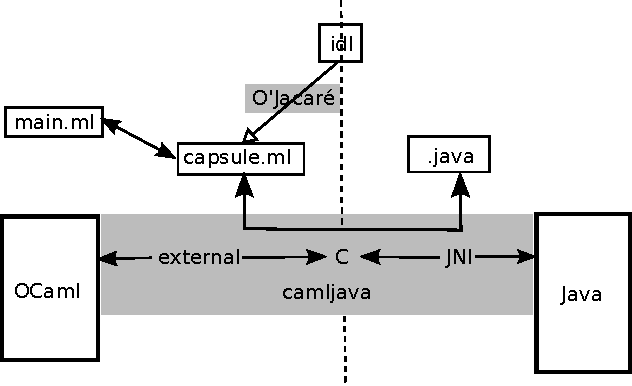
\includegraphics{schemaCamljava2.pdf}
  \caption{Schéma global de la communication par Camljava}
\end{figure}

La génération de code se fait en plusieurs passes :
\begin{itemize}
\item analyse lexicale et analyse syntaxique de l' idl donnant un AST.
\item vérification des types de l'AST, donnant un nouvel arbre nommé
  CAST (Checked AST).
\item la génération des fichiers stub java nécessaires pour un appel callback 
\item la génération à partir du CAST des classes encapsulantes dans un fichier .ml
\item la génération à partir du CAST du module .mli adapté
\end{itemize}
Ces différentes étapes seront présentées plus en profondeur.

\begin{figure}[h]
  \centering
  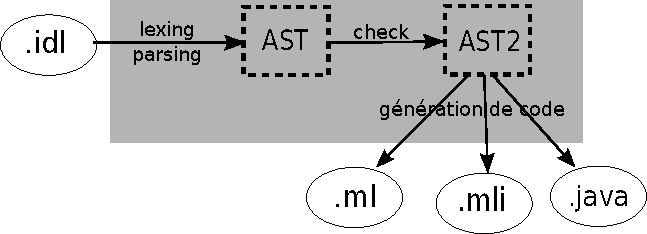
\includegraphics{schemaOjacare.pdf}
  \caption{Schéma global de la génération d'O'Jacaré}
\end{figure}

\newpage
\subsubsection{La syntaxe de l'idl}
L'IDL est défini pour la construction des interfaces entreO'Caml et
Java, il est donc défini en s'approchant de l'intersection des deux
mondes objet ( TODO : A completer : definir cette intersection )

La syntaxe du langage d'interface est donné en annexe, en utilisant la
notation BNF.

Les symboles < et > encadrent des règles optionnelles,
les terminaux sont en bleu, et les non-terminaux sont en italique.


\subsubsection{Analyse lexical, syntaxique et sémantique}
La première phase est celle d'analyse lexicale et syntaxique,
séparant l'idl en lexèmes et construisant l'AST, défini en annexe par Idl.file,
dont la structure est définie en annexe.

Vient ensuite la phase d'analyse sémantique, analysant l'AST obtenue par la
phase précédente, vérifiant si le programme est correct, et

construisant une liste de CIdl.clazz, restructurant chaque classe ou interface définie dans l'idl. 
Le module Cidl définit le nouvel AST nommé CAST allant être manipulé dans les passes de
génération de code. Il est décrit en annexe.

\subsubsection{génération stub\_file}
pour callback : génération java

\subsubsection{génération des classes encapsulantes}

Type jni

Class type

Cast JNI (up et down)

Fonction d'allocation

Capsule / souche

Downcast utilisateur (
\_downcast,
\_instance\_of)

Tableaux

Fonction d'initialisation
Classe de construction

fonctions / methodes static

\subsubsection{compilation par camljava}
interfacage C, 2 runtimes, destiné à Jni, 











%%%%%%%%%%%%%%%%%%%%%%%%%%%%%%%%%  1.2  OCaml-Java   %%%%%%%%%%%%%%%%%%%%%%%%%%%%%%%%%%%

\newpage
\subsection{OCaml-Java et la compilation de code OCaml vers du bytecode Java}
intro TODO presentation

\begin{figure}[h]
  \centering
  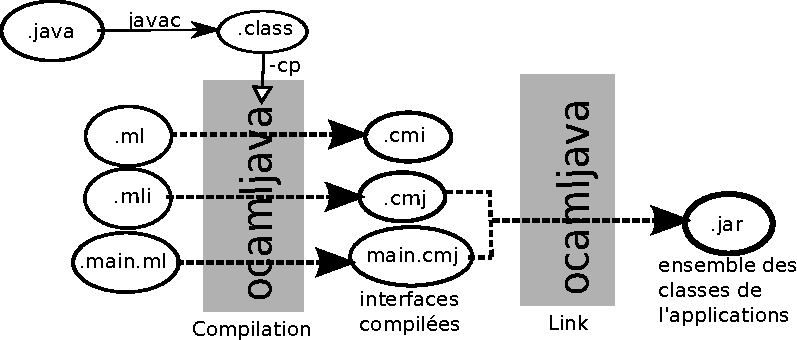
\includegraphics{schemaOCamlJava.pdf}
  \caption{Schéma global du compilateur d'OCaml-Java}
\end{figure}

\subsubsection{Accès à du code Java}
\noindent
Description des types manipulés par OCaml-Java permettant un accès au
monde de Java depuis celui d'OCaml.  

\begin{tabular}{|l|l|}
  \hline
  type Java & description et exemple \\
  \hline
  java\_constructor & signature d'un constructeur  \\
  &  "java.lang.Object()" \\
  \hline
  java\_method & signature d'une méthode \\
  & "java.lang.String.lastIndexOf(string):int"\\
  \hline
  java\_field\_get & signature d'un attribut\\
  & "mypack.Point.x:int" \\
  \hline
  java\_field\_set & signature d'un attribut\\
  & "mypack.Point.x:int" \\
  \hline
  java\_type & classe, interface ou type Array\\
  & "java.lang.String"\\
  \hline
  java\_proxy & type d'une interface\\
  & "java.lang.Comparable"\\ 
  \hline
\end{tabular}

\noindent
Description du module Java

\begin{OCamlEx}
make : 'a java_constructor -> 'a (* cree une instance d'objet *)
call : 'a java_method -> 'a (* appelle d'une methode *)
get : 'a java_field_get -> 'a (* acces a un champ, statique ou non *)
set : 'a java_field_set -> 'a (* modification du champ non statique
d'une instance d'objet *)
is_null : 'a java_instance -> bool (* teste si une instance est egale a null*)
instanceof : 'a java_type -> 'b java_instance -> bool
cast : 'a java_type -> 'b java_instance -> 'a
proxy : 'a java_proxy -> 'a
\end{OCamlEx}
Une exception est définie dans le module pour permettre d'attraper les
exceptions du côté OCaml :
\begin{OCamlEx}
exception Java_exception of java'lang'Throwable java_instance
\end{OCamlEx}



%%%%%%%%%%%%%%%%%%%%%%%%%%%%  1.3  PROBLEME, IDEE de solution   %%%%%%%%%%%%%%%%%%%%%%%%%%%%%%

\subsection{profiter des deux approches}
O'Jacaré construit les classes encapsulantes de classes
java définies par l'utilisateur, et permet ainsi l'accès aux méthodes
(d'instance ou de classe) Java en OCaml en passant par l'interface de bas niveau CamlJava.
Cette interface de bas-niveau 

OCaml-Java permet l'accès à toute l'API Java depuis OCaml TODO


\ 
\newline
Solution problèmes : TODO
- gestion de la surchage (absente en OCaml) -> renommage obligatoire
dans IDL.
- 2 runtimes vs 1 seul (-> résoud pd de communication GC et exceptions)
- gestion du typage (statype en OCaml vs dynamique en Java)
-









%%%%%%%%%%%%%%%%%%%%%%%%%%%%  2  REALISATION   %%%%%%%%%%%%%%%%%%%%%%%%%%%%%%

\section{Portage d'O'Jacaré pour OCaml-Java}


\subsection{}





\subsection{schémas de compilation actuels d'O'Jacaré}

\noindent
Nous considérons un environnement contenant les  variables suivantes, initialisées à leur valuer par défaut: 

$\rho$ = "" : le nom du \textbf{package} où trouver les classes définies.

$\Lambda$ = "" : le \textbf{nom de la classe} courant.

$\gamma$ = false : si la déclaration est une \textbf{interface}.

$\theta$ = false : si l'élément porte l'attribut \textbf{callback}.

$\alpha$ = false : si l'élément est déclaré \textbf{abstract}.

$\delta$ = "JniHierarchy.top" : la classe dont \textbf{extends} la classe courante.

$\Delta$ = [] : les interfaces qu'\textbf{implements} la classe courante.
\ %%   \rho,\Lambda,\gamma,\theta,\alpha,\delta,\Delta
\newline
\noindent


\textbf{package}
\newline
\noindent
$[\![ package\ {\color{blue}qname}\ ;\ decl^* ]\!]$$\longrightarrow$
% metttre package name dans env

$[\![ decl^* ]\!]_{\rho=qname}$ 

\ 
\newline

\textbf{ decl interface }
\newline
\noindent
$[\![{\color{blue}interface}\  name ]\!]$$\longrightarrow$

$[\![{\color{blue}class}\  name ]\!]_{\rho,\Lambda=name,\gamma=true}$

\ 
\newline

\textbf{ decl class }
\newline
\noindent
$[\![$[$ {\color{blue}callabck}$]${\color{blue} class}\  name ]\!]_{\rho,\Lambda,\gamma,\theta,\alpha}$$\longrightarrow$

$[\![{\color{blue}class}\  name ]\!]_{\rho,\Lambda=name,\gamma,\theta=true,\alpha}$

\ 
\newpage
\noindent

\textbf{ decl class}
\newline
\noindent
$[\![ {\color{blue}class}\ CLASS\ 
 {\color{blue}extends}\  E \ 
 {\color{blue}implements}\  I1,I2... \{$

 $ \ \ \ attr1; attr2; ...;$

  $\ \ \ m1; m2; ...;$

  $\ \ \ init1; init2; ...;$

 $\} ]\!]_{\rho=PACK,\ \Lambda,\ \gamma,\ \theta=false,\ \alpha=false,\ \delta,\ \Delta}\longrightarrow$
% 1 type objet t 
% 1 classe encapsulante W de type t
% 1 a n classes (Ci), sous-classes de W (1 par constructeur)
% 1 fonction instanceof pr ce type
% 1 fonction de cast pour ce type
\ 
\newline

$\Lambda=CLASS$

$\alpha=false$

$\delta=E$

$\Delta=[I1,I2,I3]$

\begin{OCaml}
   let clazz = Jni.find_class PACK/CLASS

(** type jni.obj t *)
"type _jni_jCLASS = Jni.obj"

(** classe encapsulante *)
"class type jCLASS = object 
   inherit E
   inherits jI1
   inherits jI2 ...
   method _get_jni_jCLASS : _jni_jCLASS
   end"

(** upcast jni *)
"let __jni_obj_of_jni_jCLASS (java_obj : _jni_jCLASS) =
   (Obj.magic : _jni_jCLASS -> Jni.obj) java_obj"
(** downcast jni *)
"let __jni_jCLASS_of_jni_obj =
   fun (java_obj : Jni.obj) ->
     Jni.is_instance_of java_obj clazz"
 
(* allocation *)
if not/* $\gamma$ */then
"let _alloc_jCLASS =
     fun () -> (Jni.alloc_object clazz : _jni_jCLASS)"

(* capsule wrapper *)
"class _capsule_jCLASS = fun (jni_ref : _jni_jCLASS) ->
    object (self)
      method _get_jni_jCLASS = jni_ref
      method _get_jni_jE = jni_ref
      method _get_jni_jI1 = jni_ref
      method _get_jni_jI2 = jni_ref
      inherit JniHierarchy.top jni_ref
    end"

(* downcast utilisateur *)
"let jCLASS_of_top (o : TOP) : jCLASS =
    new _capsule_jCLASS (__jni_jCLASS_of_jni_obj o#_get_jniobj)"
(* instance_of *)
"let _instance_of_jCLASS =
    in fun (o : TOP) -> Jni.is_instance_of o#_get_jniobj clazz"

(* tableaux *)
"let _new_jArray_jCLASS size =
    let java_obj = Jni.new_object_array size (Jni.find_class \"PACK/CLASS\")
    in
      new JniArray._Array Jni.get_object_array_element Jni.
        set_object_array_element (fun jniobj -> new _capsule_jCLASS jniobj)
        (fun obj -> obj#_get_jni_jCLASS) java_obj"
"let jArray_init_jCLASS size f =
    let a = _new_jArray_jCLASS size
    in (for i = 0 to pred size do a#set i (f i) done; a)"

(* inits *)
\end{OCaml}

$[\![$[$ {\color{blue}name}\ init1 $]${\color{blue} <init>} (arg*); ...\}
]\!]_{\rho,\ \Lambda,\ \gamma,\ \theta,\ \alpha,\ \delta,\ \Delta}$

$[\![$[$ {\color{blue}name}\ init2 $]${\color{blue} <init>} (arg*); ...\}
]\!]_{\rho,\ \Lambda,\ \gamma,\ \theta,\ \alpha,\ \delta,\ \Delta}$

...
\begin{OCaml}
(* fonctions et  methodes statiques*)
 
    (*TODO*)

\end{OCaml}


\
\ 
\newline
\ 
\newline
Ce tableau représente le résultat des fonctions str, jni\_type, getJni, cast sur les types lors des générations des constructeurs ou des méthodes.

\noindent
\begin{tabular}{|l|c|c|c|c|}
  \hline
  TYPE & str & jni\_type & getJni & cast \\
  \hline
  void & V & & & \\
  boolean & Z & Jni.Boolean \_pi & \_pi  & \_pi \\
  byte & B & Jni.Byte \_pi & \_pi & \_pi \\
  char & C & Jni.Char \_pi & \_pi & \_pi \\
  short & S & Jni.Short \_pi & \_pi & \_pi  \\
  int & I & Jni.Camlint \_pi & \_pi &  \_pi \\
  long & J & Jni.Long \_pi &\_pi  & \_pi \\
  float & F & Jni.Float \_pi & \_pi & \_pi \\
  double & D & Jni.Double \_pi & \_pi & \_pi \\
  string &LJava/lang/String;& Jni.Obj \_pi & Jni.string\_to\_java \_pi & \_pi \\
  pack/Obj& Lpack/Obj;& Jni.Obj \_pi & \_pi\#\_get\_jni\_jname & (\_pi : jObj) \\
  \hline
\end{tabular}
\ 
\newline
\noindent
\textbf{ inits }
\newline
\noindent
$[\![$[$ {\color{blue}name}\ INIT $]${\color{blue} <init>} (A0,
    A1, ...)]\!]_{}$$\longrightarrow$

\begin{OCaml}
"let _init_INIT =
  let id = Jni.get_methodID clazz \"<init>\" 
            \"("(toStr A0)(toStr A1)...")V\"
  in
    fun (java_obj : _jni_jCLASS) "(cast A0) (cast A1) ..." -> ...
      let _p1 = "(getJni A1)" in
      let _p0 = "(getJni A0)" in
      Jni.call_nonvirtual_void_method java_obj clazz id 
          [| "(jni\_type A0)"; "(jni\_type A1)"; ... |]

class INIT _p0 _p1 ... =
  let java_obj = _alloc_jCLASS ()
  in let _ = _init_INIT java_obj _p0 _p1 ...
    in object (self) inherit _capsule_jCLASS java_obj 
end"

\end{OCaml}
\ 
\newline
\noindent
\textbf{ attributs }
\newline
\noindent
\ 
$[\![ TYPE\ ATTR; ]\!]_{}$$\longrightarrow$

\begin{OCaml}
...
(* type class *)
"class type jCLASS =
  ...
   method set_ATTR : (j)TYPE -> unit
   method get_ATTR : unit -> (j)TYPE
   ... "
(* capsule *)
"class _capsule_jCLASS =
   let __fid_ATTR = try Jni.get_fieldID clazz \"ATTR\" "(toStr TYPE)" in
   ...
   fun (jni_ref : _jni_jCLASS) -> 
     object (self)
        method set_ATTR =
           fun "(castArg TYPE)" ->
              let _p = "(getJni TYPE)"
              in Jni.set_object_field jni_ref __fid_ATTR _p
        method get_ATTR =
        fun () ->
           (new _capsule_jCLASS (Jni.get_object_field jni_ref __fid_ATTR) :
           jCLASS)
        ...
   "
\end{OCaml}

\noindent
\textbf{ methodes }

\noindent
\begin{tabular}{|l|c|c|c|c|}
  \hline
  TYPE & str & jni\_type & getJni & cast \\
  \hline
  void & " "||V & & & \\
  boolean & Z & Jni.Boolean \_pi & \_pi  & \_pi \\
  byte & B & Jni.Byte \_pi & \_pi & \_pi \\
  char & C & Jni.Char \_pi & \_pi & \_pi \\
  short & S & Jni.Short \_pi & \_pi & \_pi  \\
  int & I & Jni.Camlint \_pi & \_pi &  \_pi \\
  long & J & Jni.Long \_pi &\_pi  & \_pi \\
  float & F & Jni.Float \_pi & \_pi & \_pi \\
  double & D & Jni.Double \_pi & \_pi & \_pi \\
  string &LJava/lang/String;& Jni.Obj \_pi & Jni.string\_to\_java \_pi & \_pi \\
  pack/Obj& Lpack/Obj;& Jni.Obj \_pi & \_pi\#\_get\_jni\_jname & (\_pi : jObj) \\
  \hline
\end{tabular}
\ 
\newline
\noindent
$[\![ TYPE METH (ARG1, ARG2, ...)]\!]_{}$$\longrightarrow$

\begin{OCaml}
...
(* type class *)
"class type jCLASS =
   ...
   method METH : ARG1 -> ARG2 -> ... -> TYPE
   ... "
(* capsule *)
"class _capsule_jCLASS =
   let __mid_METH = Jni.get_methodID clazz "mETH"
         \"("(toStr ARG1)(toStr ARG2)...")"(toStr TYPE)"\"
   ...
   in
   object (self)
"(*TODO*)"      (*method METHObj1Obj2 =
         fun (_p0 : jObj1) ->
           let _p0 = _p0#_get_jni_jObj1
           ...
             in
             (new _capsule_jObj2
               (Jni.call_"Object"_method jni_ref __mid_mETHObj1Obj2
               [| Jni.Obj _p0 |]) : jObj2)
      *)
      method METH =
         fun "(cast A0) (cast A1) ..." ->
           let _p2 = "(getJni ARG2)" in
           let _p1 = "(getJni ARG1)" in
           let _p0 = "(getJni ARG0)"
           in
             Jni.call_"(aJniType TYPE)"_method jni_ref __mid_METH
               [| "(jni\_type ARG0)"; "(jni\_type ARG1)"; ... |]
\end{OCaml}
//TODO : 
retour Obj dans methode
array
callback

 














%%%%%%%%%%%%%%%%%%%%%%%%%%%%   newOjacare   %%%%%%%%%%%%%%%%%%%%%%%%%%%%%%
\subsection{Génération de code pour Ocaml-Java}
 
Le type top manipulé sera le type d'instance objet de Ocaml-Java :
\begin{OCamlEx}
type top = java'lang'Object java_instance;;
\end{OCamlEx}

Exception :
\begin{OCamlEx}
exception Null_object of string
\end{OCamlEx}




\ 
\newline
\textbf{class}

Le schéma de compilation de base pour une classe est largement allégé. 
En effet,la fonction downcast jni est inutile, puisqu'on a la fonction Java.cast, effectuant tout le travail.

De même, l'upcast -> 

TODO : voir http://www.pps.univ-paris-diderot.fr/~henry/ojacare/doc/ojacare006.html. (** cast JNI, exporté pour préparer la fonction 'import' *)

L'allocation n'est pas non plus nécessaire, OCaml-Java gérant tout ça côté Java. 

La capsule est aussi très simplifiée, les tests d'existance des méthodes classes etc est aussi géré par COaml-Java.

\ 
\newline
\noindent
$[\![ {\color{blue}class}\ CLASS\ 
 {\color{blue}extends}\  E \ 
 {\color{blue}implements}\  I1,I2... \{$

 $ \ \ \ attr1; attr2; ...;$

  $\ \ \ m1; m2; ...;$

  $\ \ \ init1; init2; ...;$

 $\} ]\!]_{\rho,CB}\longrightarrow$
% 1 type objet t 
% 1 classe encapsulante W de type t
% 1 a n classes (Ci), sous-classes de W (1 par constructeur)
% 1 fonction instanceof pr ce type
% 1 fonction de cast pour ce type
\ 
\newline

\begin{OCaml}

(** type 'a java_instance*)
"type _jni_jCLASS = PACK'CLASS java_instance;;"

(** classe encapsulante *)
"class type jCLASS =
   object inherit E
   inherits jI1
   inherits jI2 ...
   method _get_jni_jCLASS : _jni_jCLASS
   end"

(* capsule wrapper *)
"class _capsule_jCLASS = 
  fun (jni_ref : _jni_jCLASS) ->
     let _ =
        if Java.is_null jni_ref
        then raise (Null_object "mypack/Point")
        else ()
     in

    object (self)
     (* method _get_jni_jCLASS = jni_ref
      method _get_jni_jE = jni_ref
      method _get_jni_jI1 = jni_ref
      method _get_jni_jI2 = jni_ref*)
      inherit JniHierarchy.top jni_ref
    end"

(* downcast utilisateur *)
"let jCLASS_of_top (o : TOP) : jCLASS =
    new _capsule_jCLASS (__jni_jCLASS_of_jni_obj o#_get_jniobj)"
(* instance_of *)
"let _instance_of_jCLASS =
    in fun (o : TOP) -> Jni.is_instance_of o#_get_jniobj clazz"


\end{OCaml}
\ 
\newline
\noindent
\textbf{ methodes } 



Tableau représentant les équivalents en OCaml des types Java manipulés
par OCaml-Java.
La troisième colonne représente les types manipulés par les programmes
OCaml écrit par l'utilisateur du nouvel outil.
Le problème est donc de convertir du deuxième au troisième type pour la manipulation côté OCaml et du troisième au second lors d'un appel à une fonction du module Java (un appel, un constructeur ou autre).

\begin{tabular}{|c|l|l|l|}
 \hline
TYPE IDL &type Java & type OCaml  pour OCaml-Java & type OCaml \\
& (java\_type) & (oj\_type t) & (ml\_type t) \\
 \hline
\emph{void} & void & unit & unit\\
\emph{boolean} &boolean & bool & bool\\
\emph{byte} & byte & int & int \\
\emph{char} &char & int & char\\
\emph{double} & double & float & float\\
\emph{float} & float & float & float\\
\emph{int} & int & int32 & int\\
\emph{long} & long & int64 & int\\
\emph{short} & short & int & int\\
\emph{string} & java.lang.String & java'lang'String java\_instance & string\\
\emph{pack/Obj} & pack.Obj & pack'Obj java\_instance & jObj\\
 \hline
\end{tabular}
\
\newline

Tableau associant pour chaque types de l'IDL les
fonctions utiles aux schémas de compilation manipulant ceux-ci, comme explicité ci-dessus. 

\begin{tabular}{|c|l|l|l|}
  \hline

  TYPE IDL & to\_oj\_Type ARGi & to\_ml\_type ARGi & fcast\\

  \hline
  \emph{void} &   &  & \\

  \emph{boolean} &  &  &\_pi \\

 \emph{byte} & &  &\_pi  \\

 \emph{cha}r & TODO  & TODO & \_pi \\

  \emph{short} & &  & \\

 \emph{int} & Int32.of\_int\ & Int32.to\_int & \_pi\\

 \emph{long} & Int64.of\_int & Int64.to\_int & \_pi\\

 \emph{float} & & &\_pi \\

  \emph{doubl}e & & & \_pi\\

 \emph{string} & JavaString.of\_string & JavaString.to\_string & \_pi\\

 \emph{pack/Obj} & \_pi\#\_get\_jni\_jObj & (new \_capsule\_jObj ... : jObj) & (\_pi: jObj)\\

  \hline
\end{tabular}
\ 
\newline
\ 
\newline
\noindent
$[\![\ RTYPE\ \ METH\ (TARG1,\ TARG2, ...)]\!]_{ TODO }$$\longrightarrow$

\begin{OCaml}
...
(* type class *)
"class type jCLASS =
   ...
   method METH : "(ml_type TARG1) -> (ml_type TARG2)" -> ... ->(ml_type RTYPE)
   ... "
(* capsule *)
"class _capsule_jCLASS =
   object (self)      
      method METH =
         fun "(fcast TARG0) (fcast TARG1) ..." ->
           let _p1 = "(to_oj_type TARG1)" _p1 in
           let _p0 = "(to_oj_type TARG0)" _p0
           in"
             (to_ml_type RTYPE)
             "Java.call \"PACK.CLASS.METH("(javaType TARG1),(javaType TARG2),...):(javaType RTYPE)"\" jni_ref _p0 _p1 ..."

\end{OCaml}
\ 
\newline
\noindent
\textbf{ inits }
\newline
\noindent
$[\![$[$ {\color{blue}name}\ INIT $]$\ {\color{blue}
      <init>}\ (TARG0,\ TARG1, ...)]\!]_{}$$\longrightarrow$
% 

\begin{OCaml}
"class INIT _p0 _p1 ... =
  let _p1 = "(to_oj_type TARG1)"  in
  let _p0 = "(to_oj_type TARG2)" in
  let java_obj = Java.make \"PACK.CLASS("(javaType
           TARG0),(javaType TARG1),...")\" _p0 _p1
  in 
  object (self) 
     inherit _capsule_jCLASS java_obj 
  end;;"

\end{OCaml}

\ 
\newline
\noindent
\textbf{ attributs }
\newline
\noindent
\ 
$[\![ TYPE\ \ ATTR; ]\!]_{}$$\longrightarrow$

\begin{OCaml}
...
(* type class *)
"class type jCLASS =
  ...
   method set_ATTR : "(ml_type TYPE)" -> unit
   method get_ATTR : unit -> "(ml_type TYPE)"
   ... "
(* capsule *)
"class _capsule_jCLASS =
   ...
   fun (jni_ref : _jni_jCLASS) -> 
     object (self)
     ...
        method set_ATTR =
           fun "(fcast TYPE)" ->
              let _p = "(to_oj_type TYPE)" _p
              in Java.set \"PACK.CLASS.ATTR:TYPE\" jni_ref _p
        method get_ATTR =
        fun () ->
           "(to_ml_type TYPE)" (Java.get \"PACK.CLASS.ATTR:TYPE\" jni_ref)
        ...
   "

\end{OCaml}


\section{Application et performance}







\section*{Conclusion}
\addcontentsline{toc}{section}{Conclusion}










%%%%%%%%%%%%%%%%%%%%%%%%%%%%   BIBLIOGRAPHIE   %%%%%%%%%%%%%%%%%%%%%%%%%%%%%%

\newpage
\section*{Bibliographie, références}
\addcontentsline{toc}{section}{Bibliographie, références}
[1] CHAILLOUX E., MANOURY P., PAGANO B., \emph{Développement
  d'applications avec Objective Caml}, O'Reilly
, 2000, (\url{http://www.oreilly.fr/catalogue/ocaml.html})

[2] CHAILLOUX E., HENRY G., \emph{O’Jacaré, une interface objet
  entre Objective Caml et Java}, 2004,

[3] CLERC X., \emph{OCaml-Java: Typing Java Accesses from OCaml
  Programs}, Trends in Functional Programming, Lecture Notes in
Computer Science Volume 7829,
2013, \href{http://www.cs.ru.nl/P.Achten/IFL2013/symposium_proceedings_IFL2013/ifl2013_submission_17.pdf}{lien}

[4] CLERC X., \emph{OCaml-Java: OCaml on the JVM}, Trends in
Functional Programming,
2012,\href{}{lien}

[5] CLERC X., \emph{OCaml-Java:OCaml-Java: from OCaml sources to Java bytecodes }, Trends in Functional Programming, 2012,\href{http://www.lexifi.com/ml2012/full9.pdf}{lien}

[6] Leroy X., \emph{The camljava project},
(\url{http://forge.ocamlcore.org/projects/camljava/})

[7] CLERC X.,\emph{OCaml-java : module Java} \url{http://ocamljava.x9c.fr/preview/javalib/index.html}

[8] CamlP4 (* todo *)










%%%%%%%%%%%%%%%%%%%%%%%%%%%%   ANNEXE   %%%%%%%%%%%%%%%%%%%%%%%%%%%%%%


\newpage
\section*{Annexe}
\addcontentsline{toc}{section}{Annexe}


\subsection*{BNF}
\begin{idl}
(*\class*)

file ::= (*\package*) <(*\package*)>*
  	| decl <decl>*
 
(*\package*) ::= package qname ; decl <decl>*

decl ::= (*\class*)
  	|(*\interface*)
 
(*\class*) ::= <[attributes]> <abstract> class (*\name*)
  	  < extends qname >
  	  < implements qname <, qname>* >
  	  { <class_elt ;>* }
class_elt ::= <[ attributes ]> <static> <final> type (*\name*)
            | <[ attributes ]> <static> <abstract> type (*\name*) (<args>)
            | [ attributes ] <init> (<args>)
 
(*\interface*) ::= <[ attributes ]> interface (*\name*)
  	       < extends qname <, qname>* >
  	      { <interface_elt;>* }
interface_elt ::= 
     <[ attributes ]> type (*\name*)
   | <[ attributes ]> type (*\name*) (<args>)
 
args ::= arg <, arg>*
arg ::= <[ attributes ]> type <(*\name*)>
 
attributes ::= 	attribute <, attribute>*
attribute ::= name (*\ident*)
  	    | callback
  	    | array
 
type ::= basetype
       | object
       | basetype [ ]
basetype ::= void
           | boolean
           | byte
           | char
           | short
           | int
           | long
           | float
           | double
           | string
object := qname
qname ::= (*\name*)<.(*\name*)>*
(*\name*) ::= (*\ident*)
\end{idl}

\newpage
\subsection*{Module CIdl, structure manipulée par O'Jacaré à partir de
  l'IDL}
\begin{OCaml}
(**  module CIdl  *)
type typ =
  | Cvoid
  | Cboolean (** boolean -> bool *)
  | Cchar (** char -> char *)
  | Cbyte (** byte -> int *)
  | Cshort (** short -> int *)
  | Ccamlint (** int -> int<31> *)
  | Cint (** int -> int32 *)
  | Clong (** long -> int64 *)
  | Cfloat (** float -> float *)
  | Cdouble (** double -> float *)
  | Ccallback of Ident.clazz
  | Cobject of object_type (** object -> ... *)
and object_type = 
  | Cname of Ident.clazz (** ... -> object *)
  | Cstring (** ... -> string *)
  | Cjavaarray of typ (** ... -> t jArray *) 
  | Carray of typ (** ... -> t array *) 
  | Ctop

type clazz = {
    cc_abstract: bool;
    cc_callback: bool;
    cc_ident: Ident.clazz;
    cc_extend: clazz option; (* None = top *)
    cc_implements: clazz list;
    cc_all_inherited: clazz list; (* tout jusque top ... (et avec les interfaces) sauf elle-meme. *)
    cc_inits: init list;
    cc_methods: mmethod list; (* methodes + champs *)
    cc_public_methods: mmethod list; (* methodes declarees + celles heritees *)
    cc_static_methods: mmethod list; 
  }
and mmethod_desc = 
  | Cmethod of bool * typ * typ list (* abstract, rtype, args *)
  | Cget of typ
  | Cset of typ
and mmethod = {
    cm_class: Ident.clazz;
    cm_ident: Ident.mmethod; 
    cm_desc: mmethod_desc;
  }         
and init = {
    cmi_ident: Ident.mmethod;
    cmi_class: Ident.clazz;
    cmi_args: typ list;
  }
type file = clazz list
\end{OCaml}

\subsection*{module Ident}
\begin{OCaml}
(* module Ident  *)
(* le type des identifiants de classe de l'IDL *)
type clazz = {
    ic_id: int;
    ic_interface: bool;
    ic_java_package: string list;
    ic_java_name: string;
    ic_ml_name: string;
    ic_ml_name_location: Loc.t;
    ic_ml_name_kind: ml_kind;
  }
type mmethod = {
    im_java_name: string;
    im_ml_id: int; (** entier unique pour une nom ml *)
    im_ml_name: string;
    im_ml_name_location:Loc.t;
    im_ml_name_kind: ml_kind;
  }
\end{OCaml}
\ 

\subsection*{phases de }
\ 
\newline
Type jni

\emph{MlClass.make\_jni\_type}
\newline
Class type

\emph{MlClass.make\_class\_type}
\newline
Cast JNI

\emph{MlClass.make\_jniupcast}

\emph{MlClass.make\_jnidowncast}
\newline
Fonction d'allocation

\emph{MlClass.make\_alloc}

\emph{MlClass.make\_alloc\_stub}
\newline
Capsule / souche

\emph{MlClass.make\_wrapper}
\newline
Downcast utilisateur

\emph{MlClass.make\_downcast}

\emph{MlClass.make\_instance\_of}
\newline
Tableaux

\emph{MlClass.make\_array}
\newline
Fonction d'initialisation

\emph{MlClass.make\_fun}
\newline
Classe de construction

\emph{MlClass.make\_class}
\newline
fonctions / methodes static

\emph{MlClass.make\_static}


\end{document}
